% https://tex.stackexchange.com/questions/370121/how-to-label-a-segment-in-tkz-euclide
% https://tex.stackexchange.com/questions/220503/how-to-shift-curly-brackets

\documentclass[12pt]{article}
\usepackage[utf8]{inputenc}
\usepackage{tikz, pgfplots, tkz-euclide}
\usetikzlibrary{positioning, decorations.text}

\usetikzlibrary{decorations.pathreplacing}

\begin{document}

\section*{Kepler's Second Law Derivation}

\subsection*{Definition}

A line joining a planet and the Sun sweeps out equal areas during equal intervals of time.

\subsection*{Derivation}

For this line to sweep out equal area during equal time,
the rate at which the area changes, $\frac{dA}{dt}$ must stay constant.
One ``infinitely'' small slice of the area of a planet's elliptical orbit may be represented as
a triangle

$$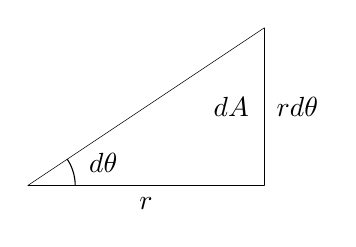
\begin{tikzpicture}

    \tkzDefPoint(0,0){A}
    \tkzDefPoint(3,2){B}
    \tkzDefPoint(3,0){C}

    \tkzDrawSegments(A,B B,C C,A)

    \tkzLabelSegment[below=1pt](C,A){$r$}
    \tkzLabelSegment[right=1pt](B,C){$rd\theta$}

    \tkzMarkAngle[size=0.60cm](C,A,B)
    \tkzLabelAngle(C,A,B){$d\theta$}

    \tkzLabelSegment[left=2pt](B,C){$dA$}

  \end{tikzpicture}$$

with base $r$, height $rd\theta$, and area $dA$ (recall that arc length is $rd\theta$).\\
Recall the equation for the area of a triangle,
$$A = \frac{1}{2}bh .$$
Substituing the givens from our infinitely small slice above, we get
$$dA = \frac{1}{2} (r) (rd\theta) .$$
Divide both sides by dt (keep in mind that $r$ is constant)
$$\frac{dA}{dt} = \frac{1}{2} (r) (r \frac{d\theta}{dt}) ,$$
which simplies to
$$\frac{dA}{dt} = \frac{1}{2} r v_t .$$
Recall that angular momentum is
$$L = mrv_t$$
and is a conserved quantity. Substiting L into our area gets
$$\frac{dA}{dt} = \frac{L}{2m} .$$
We can then rearrange and solve the differential equation
$$\int_{}^{} \,dA = \int_{}^{} \frac{L}{2m} \,dt $$
which shows us that
$$A = \frac{L}{2m} T .$$
This shows us a directly proportional relationship between the area $A$ and time $T$.
\end{document}
